\documentclass{article}
\usepackage{amsmath,amsthm,amsfonts,amssymb,enumitem,graphicx,fullpage,subfig,mathtools,listings,float,fancyvrb}

\graphicspath{{images/}}

\setlength{\parindent}{0pt}

\begin{document}

\title{Using Mixed Effects Models to Analyze Corn and Soybean Crop Areas in Iowa Based on Satellite Data}
\author{Samayita Bhattacharjee
\and Emily Chang
\and Michael Chen
\and Russell Okino}

\maketitle

\section{Summary of Reference Paper and Data}

In their 1988 paper, Battese, Harter, and Fuller \cite{battese} analyzed data on crop areas from 12 Iowa counties (obtained from the 1978 June Enumerative Survey of the U.S. Department of Agriculture) and satellite data from the 1978 growing season. The primary purpose of their study was to build a model that can predict the area (in hectares) of corn and soybeans in these counties based on satellite data identifying the number of ``pixels" (about 0.45 hectares each) classified as either corn or soybean in each ``segment" (about 250 hectares) of data.
\medbreak

In total, Battese et al. had data from 37 segments spread across the 12 counties; the number of sampled segments per county ranged from one to six. However, one of the sample segments from Hardin county appeared to have mis-entered data; therefore, that sample segment was removed in our analyses. See Figure \ref{cornplot} and Figure \ref{soyplot} for plots of the data with the mis-entered observation marked by an `X'. The exact area of corn and soybeans in the segments were obtained by interviewing farm operators, and USDA procedures were used to obtain the pixel counts of corn and soybeans for each segment based on the satellite data. The overall dataset contains the following information:

\begin{itemize}
	\item The total number of segments in each county and the number of sampled segments in each county
	\item The exact area (in hectares) of corn and soybeans in each sample segment
	\item The number of pixels classified as corn and soybeans in each sample segment
	\item The mean number of pixels per segment classified as corn and soybeans for each county
\end{itemize}

The following nested-error regression (NER) model was proposed by Battese et al. to explain the relationship between actual crop area of corn (or soybeans) and the number of pixels classified as corn and soybeans based on the satellite data:
\begin{equation}
y_{ij}=\beta_0+\beta_1x_{1ij}+\beta_2x_{2ij}+v_i+e_{ij}
\end{equation}
$i=1,\dots,12$; $j=1,\dots,n_i$ where $n_i$ is the number of sample segments in the $i$th county; $x_{1ij}$ and $x_{2ij}$ are the number of pixels classified as corn and soybeans, respectively, in the $j$th segment of the $i$th county; $\beta_0,\beta_1,\beta_2$ are unknown fixed effects; $v_i$'s are the random effects associated with the $i$th county; $e_{ij}$ are the sampling errors associated with the $j$th segment of the $i$th county. The county random effects and sampling errors are assumed to be independent of each other with $v_i \sim \mathcal N(0,\sigma_v^2)$ and $e_{ij} \sim \mathcal N(0,\sigma_e^2)$.
\medbreak

Then, a further model was proposed to relate the mean area of crops (either corn or soybean) per segment for each county to the mean number of pixels classified as corn and soybeans per segment in that county as follows:
\begin{equation}
\bar y_{i\cdot} = \beta_0+\beta_1\bar x_{1i\cdot}+\beta_2\bar x_{2i\cdot}+v_i+\bar e_{i\cdot}
\end{equation}
$\bar y_{i\cdot}:=\frac{1}{n_i}\sum_{j=1}^{n_i}y_{ij}$ is the mean area of crops per segment for county $i$;  $\bar x_{1i\cdot}:=\frac{1}{n_i}\sum_{j=1}^{n_i}x_{1ij}$ is the mean number of pixels classified as corn in county $i$; $\bar x_{2i\cdot}:=\frac{1}{n_i}\sum_{j=1}^{n_i}x_{2ij}$ is the mean number of pixels classified as soybeans in county $i$; $\bar e_{i\cdot}:=\frac{1}{n_i}\sum_{j=1}^{n_i}e_{ij}$ is the sample mean of the error terms for the $i$th county.
\medbreak

Finally, Battese et al. expressed the population mean area of crops (either corn or soybean) as
\begin{equation}
\theta_i = \beta_0+\beta_1\bar X_{1i}+\beta_2\bar X_{2i}+v_i\ ,
\end{equation}
where $\bar X_{1i}$ and $\bar X_{2i}$ are the population mean numbers of pixels classified as corn and soybeans, respectively, in county $i$. These values are known since the data includes satellite classification for all the segments in each county.
\medbreak

A practical reason for building the models in this way is that it would be tedious and expensive to manually measure the actual area of corn and soybeans in every county. Therefore, it would be beneficial if we can use satellite data to accurately estimate the mean areas without having to actually measure them. The authors presumed that the random errors may be correlated within counties since specific counties may have certain defining characteristics that make it easier or harder to get accurate measurements, so a county-specific random effect is included in the model to account for this.
\medbreak

Some non-obvious things:
\begin{enumerate}
	\item It seems that the authors considered their `base' model to be model (3). That is, they did not consider models fewer than two predictors. Intuitively, this is somewhat odd since it is reasonable to think that corn response may only be influenced by corn pixel data and soy response only be influence by soy pixel data. In fact, in our following analyses, we did consider one-predictor models, and those turned out to be better than (3) from an AIC/BIC perspective.
	\item The way the authors set the model up assumed that observations within the same county are correlated, but that observations across counties are independent. However, given the nature of the data, it is not apparent that county designation should make a discernible difference in the measurements. Perhaps there are reasons why observations from certain counties may be more or less accurate, but the authors did not explicitly mention this. Additionally, if there indeed are correlations between geographically-close observations, we are not sure that county lines are the best way to separate the data since county lines are manmade and somewhat arbitrary. All of the counties present in the study are right next to each other, so it may be just as reasonable to consider the region as one large `county'. See Figure \ref{IowaCounties} for a map of the counties.
	\item The authors considered only corn and soybeans data. However, are there other common crops planted in those Iowa counties? How about landscape-related information, such as elevation of the ground at measurement points? Such data could potentially be helpful in fitting the model. It is possible that corn and soybeans comprise the vast majority of crops grown in those counties, but this is not explicitly mentioned in the paper.
\end{enumerate}

\section{Model Selection}

In this section, we are interested in fitting model (1) with up to quadratic terms in the model. The variables for consideration are the following: $x_{1ij},x_{2ij},x_{1ij}^2,x_{2ij}^2,x_{1ij}x_{2ij}$. In total, we fit 21 models ranging from the null model (with no $x$ predictors) to the full model (with all predictors up to quadratic terms plus interaction term) and computed the AIC and BIC of each model. Let $y_{ij}^C$ denote the responses for the corn data and $y_{ij}^S$ denote the responses for the soy data. Similar notation will be used in the rest of this report to designate data/parameters relating to corn and soybeans, respectively.
\medbreak

It turns out that the model with the lowest AIC and BIC where corn area is the response has only $x_{1ij}$ as a predictor; i.e., only the corn pixel data. The fitted model is as follows:
\begin{equation}
y_{ij}^C=-1.039+0.414x_{1ij}+v_i^C+e_{ij}^C
\end{equation}

Similarly, the model with the lowest AIC and BIC where soy area is the response includes only $x_{2ij}$ as a predictor; i.e., only the soy pixel data. The fitted model is as follows:
\begin{equation}
y_{ij}^S=-3.185+0.473x_{2ij}+v_i^S+e_{ij}^S
\end{equation}

In fact, in the original model (1) selected by Battese et al., when fitting the models with corn area and soy area (respectively) as the response, the predictor based on the ``other" crop's pixel data is not significant at level $\alpha=0.01$. That is, when corn area is the response and we fit model (1), the estimate for $\beta_2$ is insignificant; and when soy area is the response in the same model, the estimate for $\beta_1$ is insignificant. This, along with the results of the AIC and BIC analyses, suggests that it would be practical to include only one predictor in the final model for each response. Furthermore, the principle of parsimony suggests that a simpler model should be preferred.
\medbreak

The formulas for AIC and BIC are
\[
AIC = -2\log \hat L + 2p \qquad \text{and} \qquad BIC = -2\log \hat L + p\log n\ ,\
\]
where $\hat L$ is the likelihood function of the model (evaluated at REML estimates). From this, it is apparent that the only difference between the two information criterion is the multiplier for $p$ in the second term. When $n\geq8$, $\log n > 2$ and so in general BIC tends to pick models of smaller size than AIC. In this case, they pick the same model.
\medbreak

Therefore, the version of Equation (3) that we will assess in the next section only includes one predictor for each response. The models are:
\begin{align}
\theta_i^C=-1.039+0.414\bar X_{1i}+v_i^C \\
\theta_i^S=-3.185+0.473\bar X_{2i}+v_i^S
\end{align}

\subsection{Discussion on Effective Sample Size}

In using the BIC criterion for model selection, we implicitly used $n=36$ for the sample size (i.e., the total number of sample segments used in model fitting). However, observations from the same county are likely to be correlated - this is part of the reason why we are fitting a random effects model in the first place. Therefore, based on assumptions presented in the model, the actual effective sample size should be somewhere between the number of counties (12) and the sample size (36). 
\medbreak

One proposed formula \cite{effsize} for the effective sample size is
\begin{equation}
n_\text{eff} = \frac{n}{1+(n-1)\rho}\ ,
\end{equation}
where $n$ is the sample size and $\rho$ is the correlation between observations in the sample. Note that if $\rho=0$ (i.e., all observations are uncorrelated), then $n_\text{eff}=n$. And when $\rho=1$ (i.e., all observations are perfectly correlated), then $n_\text{eff}=1$. These values fit intuitively with our understanding of ``effective" sample size.
\medbreak

That being said, in our dataset, the correlation between all observations is not constant (correlation is assumed to only exist within counties). Due to the uncertainty in applying this formula, we decided to use the actual sample size $n=36$ in our procedure. In any case, even using $\log(12)$ as the penalty multiplier for BIC (i.e., taking all observations in each county to be totally correlated when calculating effective sample size), the chosen models are still the same as (4) and (5).

\section{EBLUPs of the Population Mean Crop Areas}

The EBLUPs of the mixed effects are the estimated values of (6) and (7). Note that in those equations, we have already substituted in the REML estimates of $\boldsymbol\beta$. The EBLUPs of the random effects can be obtained from R's \texttt{ranef} function and are identical to those calculated using the conditional normal mean formula. Plugging these values into (6) and (7), we get the following EBLUPs for the mean hectares of corn/soy per segment for each county:

\begin{verbatim}
        County EBLUP corn EBLUP soy
1  Cerro Gordo   125.7571  78.23309
2     Hamilton   127.4073  93.24168
3        Worth   108.1242  87.46083
4     Humboldt   111.8056  81.91509
5     Franklin   143.1815  66.36608
6   Pocahontas   112.9011 113.20287
7    Winnebago   115.3597  97.36649
8       Wright   123.3955 112.57477
9      Webster   114.3663 109.95843
10     Hancock   123.6049 100.47832
11     Kossuth   108.4556 119.06613
12      Hardin   139.4874  75.01237
\end{verbatim}

Visualizations of these results can be seen in Figures \ref{cornEBLUPs} and \ref{soyEBLUPs}.

\section{MSPE Estimation: SUMCA Method}

It is of interest to estimate the prediction error of these mixed effects $\theta_i$. Due to the form of the estimator, it is difficult to get an analytic expression. Therefore, we use the SUMCA method to obtain estimates of the MSPEs.

\subsection{Overview of General SUMCA Method}

Suppose $\boldsymbol\eta$ is a mixed effect and that $\hat{\boldsymbol\eta}$ is a predictor of it. The MSPE of $\hat{\boldsymbol\eta}$ is given by
\[
\text{MSPE}(\hat{\boldsymbol\eta})=\mathbb E[\mathbb E[(\hat{\boldsymbol\eta}-\boldsymbol\eta)^2|\mathbf y]]\ .
\]
Denote $\mathbf a(\mathbf y,\boldsymbol\psi):=[\hat{\boldsymbol\eta}-\mathbf a_1(\mathbf y,\boldsymbol\psi)]^2+\mathbf a_2(\mathbf y,\boldsymbol\psi)$ where $\mathbf a_1(\mathbf y,\boldsymbol\psi)=\mathbb E[\boldsymbol\eta|\mathbf y]$ and $\mathbf a_2(\mathbf y,\boldsymbol\psi)=\text{Var}(\boldsymbol\eta|\mathbf y)$. Under the assumption that $\hat{\boldsymbol\psi}$ is consistent and $\hat{\boldsymbol\eta}=\mathbf a_1(\mathbf y,\hat{\boldsymbol\psi})$, we have the following simplification:
\[
\mathbf a(\mathbf y,\hat{\boldsymbol\psi}) = \mathbf a_2(\mathbf y,\hat{\boldsymbol\psi}) = \text{Var}[\boldsymbol\eta|\mathbf y]\vert_{\boldsymbol\psi=\hat{\boldsymbol\psi}}
\]
Then, to estimate the MSPE, we can use
\[
\widehat{\text{MSPE}} = \mathbf a_2(\mathbf y,\hat{\boldsymbol\psi})+\mathbb E[\mathbf a(\mathbf y,\boldsymbol\psi)]-\mathbb E[\mathbf a(\mathbf y,\hat{\boldsymbol\psi})]\ .
\]
Using Monte Carlo methods, this is approximated by
\[
\text{MSPE}(\hat{\boldsymbol\eta})\approx\mathbf a_2(\mathbf y,\hat{\boldsymbol\psi}) + \frac{1}{K}\sum_{k=1}^{K} \{\mathbf a(\mathbf y_{[k]},\hat{\boldsymbol\psi})-\mathbf a(\mathbf y_{[k]},\hat{\boldsymbol\psi}_{[k]})\}\ ,
\]
where $\hat{\boldsymbol\psi}$ is the estimated vector of paramters (based on the fitting of the original model on $\mathbf y$), $\mathbf y_{[k]}$ is the vector of replicates from the $k$th Monte Carlo sample, and $\hat{\boldsymbol\psi}_{[k]}$ is the estimated vector of parameters based on each new sample $\mathbf y_{[k]}$.
\medbreak


\subsection{SUMCA Method in Our Project}

Our expressions for the mixed effects of the corn and soybeans populations means are:
\begin{align}
&\theta_i^C=\beta_0^C+\beta_1^C\bar{X}_{1i}+v_i^C \\
&\theta_i^S=\beta_0^S+\beta_2^S\bar{X}_{2i}+v_i^S
\end{align}
Compared to the population mean area model (3), note that since the responses in (9) and (10) are separated for corn and soy, each one only has its corresponding predictor in the expression. One can think of the parameter for the other predictor being equal to zero since it was insignificant in the model selection process.
\medbreak

We will change the vector of parameters to take the model selection into account. Let $\boldsymbol\psi = (M,\boldsymbol\lambda)$ be our vector of parameters. Here $M$ denotes the model being used, i.e. thinking of the model as a parameter. Note that with the possible variables for selection being `corn', `soy', `corn2', `soy2', and `corn:soy', $M$ is one of $2^5=32$ possible models. $\boldsymbol\lambda=(\beta_0,\beta_1,...,\beta_5,\sigma_v^2,\sigma_e^2)$ denotes the standard parameter vector. If the model $M$ does not include a variable, the corresponding $\beta$ for that variable will be 0.

\subsubsection{Part I: Nonparametric Bootstrap}

In order to generate Monte Carlo samples, we need to first specify the model because we need to know which of the fixed effects to include while sampling. In order to choose models to sample from, we will assign probabilities of using each model with the following nonparametric bootstrap procedure:
\medbreak

For $b$ in 1 to 1000:
\begin{enumerate}
	\item Draw samples of size $n=36$ with replacement from the triples of observed data $\{(y_{ij},x_{ij},z_{ij}):i=1,...,12;j=1,...,n_i\}$. $y_{ij}$ denotes the response in the $ij$th county. $x_{ij}$ and $z_{ij}$ are the corresponding data for the fixed and random effects.  Call the bootstrap sample $(\mathbf y^{(b)},\mathbf X^{(b)},\mathbf Z^{(b)})$. Note that this procedure may result in some counties not being represented at all in the bootstrap sample. Our model selection only chooses the fixed effects, so this is OK.
	\item Fit all the models: $m_1,\dots,m_{32}$ on the bootstrap samples, i.e. $\mathbf y^{(b)} \sim \mathbf X^{(b)} + \mathbf Z^{(b)}$. Examine the AIC/BIC of each model and record which model was optimal for the bootstrap data.
\end{enumerate}
Now define the probability of selecting the $\ell$th model as:
\[
p_\ell = \frac{\# \text{times model } \ell \text{ selected}}{1000}\ .
\]
So the probability of choosing any of the 32 models is the proportion of times it was the optimal model from the bootstrap procedure.

\subsubsection{Part II: Monte Carlo Sampling}

Note that the vector of random effects $\mathbf v$ and $\mathbf y$ are jointly normal:
\[
\begin{pmatrix}\mathbf v \\ \mathbf y \end{pmatrix} \sim \mathcal N \left(\begin{pmatrix}\mathbf 0 \\ \mathbf X\boldsymbol\beta \end{pmatrix}, \begin{pmatrix}\mathbf G & \mathbf G\mathbf Z^T \\ \mathbf Z\mathbf G & \mathbf V \end{pmatrix}\right)\ ,
\]
where $\mathbf G=\sigma_v^2 \mathbf I_{12}$ (note that $\mathbf G$ is symmetric), $\mathbf Z=\text{diag}(\boldsymbol{1}_{n_1},...,\boldsymbol{1}_{n_{12}})$, $\mathbf V=\sigma_v^2 \mathbf I_{36} + \sigma_e^2 \mathbf Z\mathbf Z^T$.
\medbreak

Additionally, under the framework of using the model as a parameter, we have
\begin{align*}
\mathbf a(\mathbf y,\hat{\boldsymbol\psi}_\ell) &= \mathbf a_2(\mathbf y,\hat{\boldsymbol\psi}_\ell) \\
&= \text{Var}(\boldsymbol\theta|\mathbf y) \\
&= \text{Var}(\mathbf v|\mathbf y) \\
&= \hat{\mathbf G}-\hat{\mathbf G}\mathbf Z^T \hat{\mathbf V}^{-1} \mathbf Z \hat{\mathbf G}\ ,
\end{align*}
where $\hat{\boldsymbol\psi}_\ell$ is the estimated parameter vector when model $\ell$ is selected.
\medbreak

The Monte Carlo sample size we chose was $K=3000$. The reason for this is that the estimates for the MSPEs appear to stabilize at that number of simulations (see Figure \ref{montecarlo}). For $k$ in 1 to 3000:
\begin{enumerate}
	\item Randomly select a model $M_k$ by using the probabilities found from the nonparametric bootstrap.
	\item Generate a sample of size $n=36$ under the model $M_k$. This includes generating $\tilde{\mathbf v}_k \sim \mathcal N(\mathbf 0,\hat{\sigma}_v^2 \mathbf I_{12})$, $\tilde{\mathbf e}_k \sim \mathcal N(\mathbf 0, \hat{\sigma}_e^2 \mathbf I_{36})$ and computing $\mathbf y_{[k]}=\mathbf X\hat{\boldsymbol\beta} + \tilde{\mathbf v}_k + \tilde{\mathbf e}_k$. Here all of the estimated parameters used come from the fit of model $M_k$ on the original data.
	\item Fit all 32 possible models using the sample $\mathbf y_{[k]}$. Determine the optimal model according to AIC/BIC.
	\item Using the optimal model, compute $\hat{\boldsymbol\psi}_{\ell[k]}$. Also compute $\mathbf a_2(\mathbf y_{[k]},\hat{\boldsymbol\psi}_{\ell[k]})$. (This is $\hat{\mathbf G}-\hat{\mathbf G}\mathbf Z^T \hat{\mathbf V}^{-1} \mathbf Z \hat{\mathbf G}$ as above, but with the estimates of the variance matrices coming from $\hat{\boldsymbol\psi}_{\ell[k]}$ as opposed to just $\hat{\boldsymbol\psi}$.)
	\item Note that even though the values of $\mathbf a_2(\mathbf y_{[k]},\hat{\boldsymbol\psi}_\ell)$ and $\mathbf a_2(\mathbf y,\hat{\boldsymbol\psi}_\ell)$ are equal, $\mathbf a_2(\mathbf y_{[k]},\hat{\boldsymbol\psi}_\ell)$ depends on the model selected at the $k$th simulation. Then compute $\mathbf a_2(\mathbf y_{[k]},\hat{\boldsymbol\psi}_\ell)-\mathbf a_2(\mathbf y_{[k]},\hat{\boldsymbol\psi}_{\ell[k]})$. Store these values.
\end{enumerate}

Now define 
\[
\mathbf a^* = \sum_{\ell=1}^{32} \mathbf a_2(\mathbf y,\hat{\boldsymbol\psi}_\ell)p_\ell\ ,
\]
i.e. $\mathbf a^*$ is a weighted average of the $\mathbf a_2(\mathbf y,\hat{\boldsymbol\psi}_\ell)$ with the weights being the probabilities of selecting the corresponding model. This is the leading term of the SUMCA estimator.
\medbreak

Our SUMCA estimators of the MSPE are the diagonal elements of the 12x12 matrix
\[
\mathbf a^* + \frac{1}{K}\sum_{k=1}^K [\mathbf a_2(\mathbf y_{[k]},\hat{\boldsymbol\psi}_\ell)-\mathbf a_2(\mathbf y_{[k]},\hat{\boldsymbol\psi}_{\ell[k]})]\ .
\]

\subsection{MSPE Results}

The results of the MSPE calculations are as follows. The counties are numbered in order of appearance in the paper; i.e., county 1 is Cerro Gordo and county 12 is Hardin.
\medbreak

For the corn response:

\begin{verbatim}
County MSPE.corn.AIC MSPE.corn.BIC
     1      80.84379      80.45623
     2      80.84379      80.45623
     3      80.84379      80.45623
     4      56.75946      57.28858
     5      43.45988      44.18791
     6      43.45988      44.18791
     7      43.45988      44.18791
     8      43.45988      44.18791
     9      35.11237      35.86118
    10      29.40816      30.12596
    11      29.40816      30.12596
    12      29.40816      30.12596
\end{verbatim}

For the soy response:

\begin{verbatim}
County MSPE.soy.AIC MSPE.soy.BIC
     1    118.20186    117.52183
     2    118.20186    117.52183
     3    118.20186    117.52183
     4     75.20178     74.81364
     5     54.78997     54.54561
     6     54.78997     54.54561
     7     54.78997     54.54561
     8     54.78997     54.54561
     9     42.97635     42.81266
    10     35.30254     35.18841
    11     35.30254     35.18841
    12     35.30254     35.18841
\end{verbatim}

A visualization of these results can be found in Figures \ref{cornEBLUPs2} and \ref{soyEBLUPs2}. Note that the prediction intervals are smaller for the counties that had more observations, which is an intuitive result. For the three counties that only had one observation, the intervals are very wide since there is not much data to go off of.

\section{Conclusion}

In producing this report, we differed from the original authors' methodology in that we considered one-predictor models for the corn and soybean crop area responses that only included the crop's respective predictor (i.e. a model with only the corn pixel data as a predictor for the corn response and a model with only the soy pixel data as a predictor for the soy response). It turns out that using both the AIC and BIC criteria, these models are preferred compared to the authors' model that includes both the corn and soy pixel data as predictors for each response. This is an intuitive result since it would seem natural that only each crop's respective pixel data would be relevant to its area.
\medbreak

Random effects were used in our models to account for the correlation between data from the same county. We then used our models to get EBLUPs for the population mean crop areas per segment per county for each of the two crops. It is of interest to get an estimate of the prediction errors; we used the SUMCA method to produce these estimates. Due to some of the counties having very few observations in the sample, the prediction errors for those counties are very large and perhaps not particularly useful. However, for the counties with five observations, the prediction bands are relatively small. It is interesting to note that all the prediction bands for both crop responses include all the original data points within the bands. Furthermore, the AIC and BIC intervals are extremely similar.
\medbreak

From a practical standpoint, these analyses are useful since it is expensive and time-consuming to manually measure crop areas in farmland. Being able to use satellite data to accurate predict the crop areas is very useful. In this report, which is based on the data of Battese et al.'s original 1988 paper, only corn and soybean crop data were considered. However, it is reasonable to expect that similar methodology may be applied to different crop types as well, and can be used in other states to similarly save time and money in estimating crop areas.

\begin{thebibliography}{1}
	\bibitem{battese} Battese, G. E., Harter, R. M., \& Fuller, W. A. (1988). An error-components model for prediction of county crop areas using survey and satellite data. \textit{Journal of the American Statistical Association, 83}(401), 28-36.
	
	\bibitem{effsize} Wikipedia contributors. (2018, September 10). Effective sample size. In \textit{Wikipedia, The Free Encyclopedia}. Retrieved 19:44, March 18, 2019, from https://en.wikipedia.org/w/index.php?title=Effective\_sample \_size\&oldid=858933935
	
	\bibitem{book} Jiang, J. (2007). \textit{Linear and generalized linear mixed models and their applications}. Springer Science \& Business Media.
	
	\bibitem{lectures} Jiang, J. (2018). STA 232B lecture slides. University of California, Davis.
	
\end{thebibliography}


\newpage
\section{Appendix}

\subsection{Figures}

\begin{figure}[H]
	\centering
	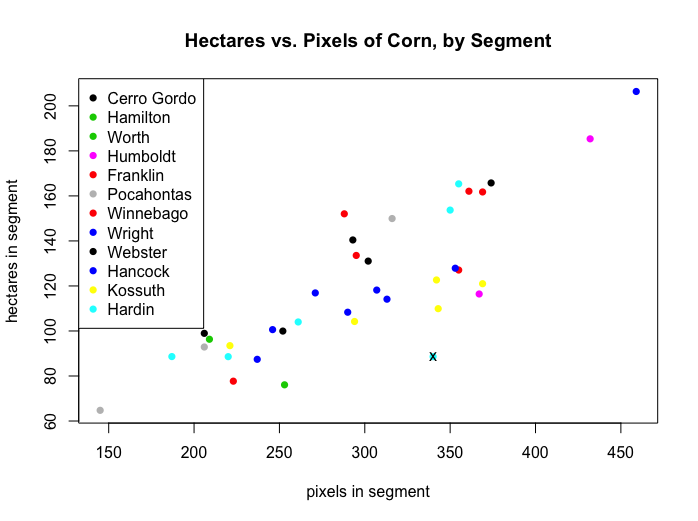
\includegraphics[scale=0.45]{cornplot}
	\caption{Corn data. The removed data point is marked with an `X'.}
	\label{cornplot}
\end{figure}

\begin{figure}[H]
	\centering
	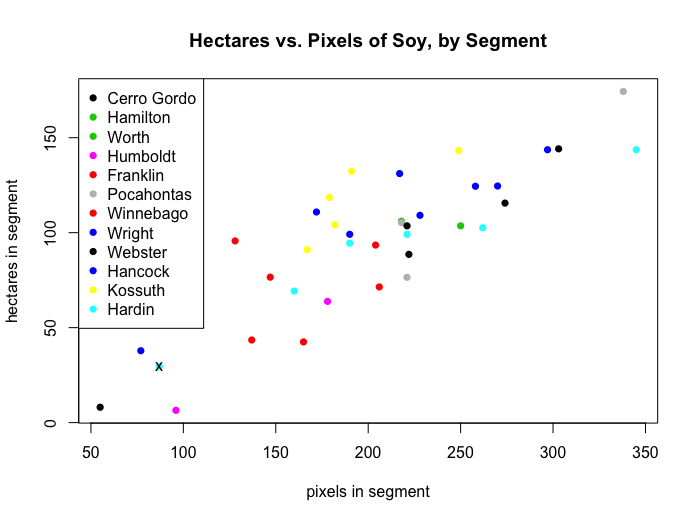
\includegraphics[scale=0.45]{soyplot}
	\caption{Soy data. The removed data point is marked with an `X'.}
	\label{soyplot}
\end{figure}

\begin{figure}[H]
	\centering
	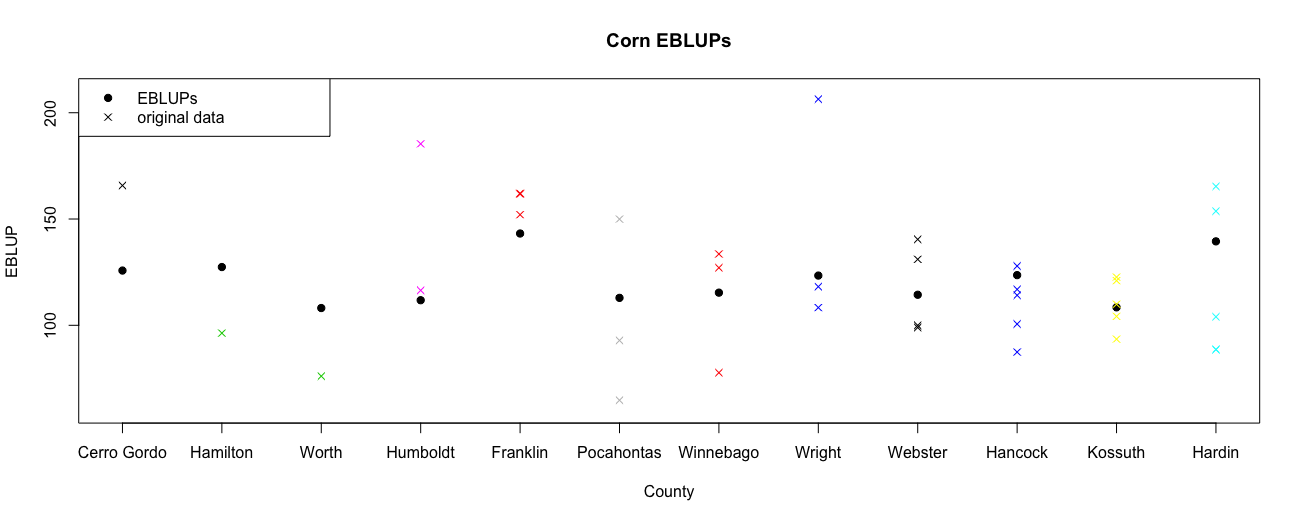
\includegraphics[scale=0.4]{cornEBLUPs}
	\caption{EBLUPs of the corn areas for each county.}
	\label{cornEBLUPs}
\end{figure}

\begin{figure}[H]
	\centering
	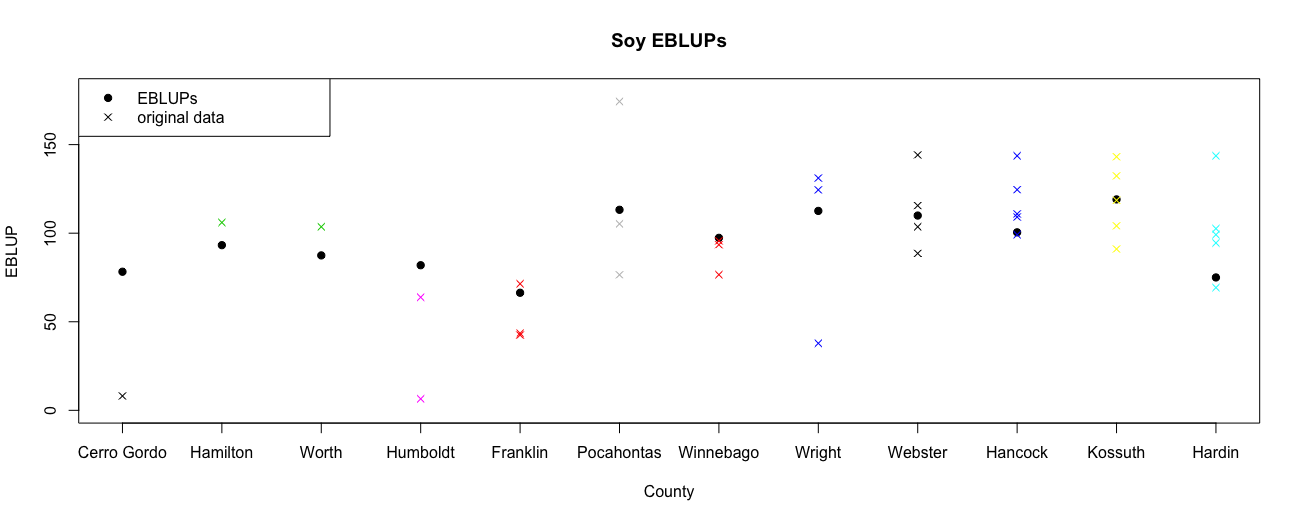
\includegraphics[scale=0.4]{soyEBLUPs}
	\caption{EBLUPs of the soy areas for each county.}
	\label{soyEBLUPs}
\end{figure}

\begin{figure}[H]
	\centering
	
\includegraphics[scale=0.4]{iowacounties}
	\caption{Map of the counties in Iowa. The ones present in the study are outlined in red.}
	\label{IowaCounties}
\end{figure}

\begin{figure}[H]
	\centering
	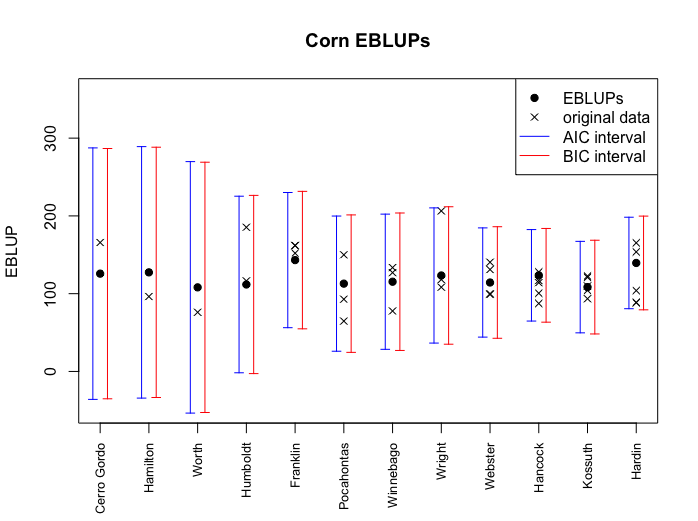
\includegraphics[scale=0.4]{cornEBLUPs2}
	\caption{EBLUPs of the corn areas for each county with prediction intervals.}
	\label{cornEBLUPs2}
\end{figure}

\begin{figure}[H]
	\centering
	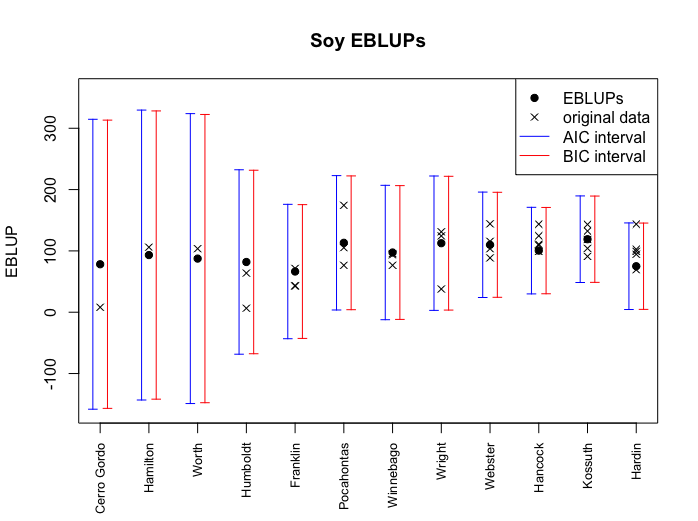
\includegraphics[scale=0.4]{soyEBLUPs2}
	\caption{EBLUPs of the soy areas for each county with prediction intervals.}
	\label{soyEBLUPs2}
\end{figure}

\begin{figure}[H]
	\centering
	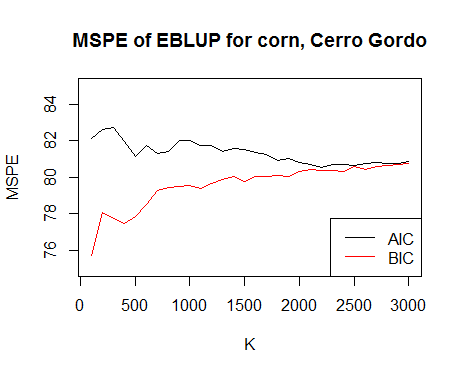
\includegraphics[scale=0.8]{montecarlo}
	\caption{Convergence of MSPE estimate for Cerro Gordo with different values of $K$.}
	\label{montecarlo}
\end{figure}

\subsection{Code}

\begin{Verbatim}[fontsize=\tiny]
rm(list = ls())
library(car)
library(lme4)

############################################################ 
# HELPER FUNCTIONS 
############################################################ 

# Take a dataframe and return IC estimates for all 32 models for corn
subsets.corn.ICs <- function(mydata){
# Models for corn
fit.c.none <- lmer(hectares.corn ~ (1|county), data = mydata)

fit.c.c <- lmer(hectares.corn ~ pixels.corn + (1|county), data = mydata)
fit.c.s <- lmer(hectares.corn ~ pixels.soy + (1|county), data = mydata)
fit.c.i <- lmer(hectares.corn ~ pixels.corn:pixels.soy + (1|county), data = mydata)
fit.c.c2 <- lmer(hectares.corn ~ I(pixels.corn^2) + (1|county), data = mydata)
fit.c.s2 <- lmer(hectares.corn ~ I(pixels.soy^2) + (1|county), data = mydata)

fit.c.cs <- lmer(hectares.corn ~ pixels.corn + pixels.soy + (1|county), data = mydata)
fit.c.ci <- lmer(hectares.corn ~ pixels.corn + pixels.corn:pixels.soy + (1|county), data = mydata)
fit.c.si <- lmer(hectares.corn ~ pixels.soy + pixels.corn:pixels.soy + (1|county), data = mydata)
fit.c.cc2 <- lmer(hectares.corn ~ pixels.corn + I(pixels.corn^2) + (1|county), data = mydata)
fit.c.cs2 <- lmer(hectares.corn ~ pixels.corn +I(pixels.soy^2) + (1|county), data = mydata)
fit.c.ss2 <- lmer(hectares.corn ~ pixels.soy +I(pixels.soy^2) + (1|county), data = mydata)
fit.c.sc2 <- lmer(hectares.corn ~ pixels.soy +I(pixels.corn^2) + (1|county), data = mydata)
fit.c.ic2 <- lmer(hectares.corn ~ I(pixels.corn^2) + pixels.corn:pixels.soy + (1|county), data = mydata)
fit.c.is2 <- lmer(hectares.corn ~ I(pixels.soy^2) + pixels.corn:pixels.soy + (1|county), data = mydata)
fit.c.c2s2 <- lmer(hectares.corn ~ I(pixels.corn^2) + I(pixels.soy^2) + (1|county), data = mydata)

fit.c.csi <- lmer(hectares.corn ~ pixels.corn*pixels.soy + (1|county), data = mydata)
fit.c.csc2 <- lmer(hectares.corn ~ pixels.corn + pixels.soy + I(pixels.corn^2) + (1|county), data = mydata)
fit.c.css2 <- lmer(hectares.corn ~ pixels.corn +pixels.soy + I(pixels.soy^2) + (1|county), data = mydata)
fit.c.cic2 <- lmer(hectares.corn ~ pixels.corn + pixels.corn:pixels.soy + I(pixels.corn^2) + (1|county), data = mydata)
fit.c.cis2 <- lmer(hectares.corn ~ pixels.corn + pixels.corn:pixels.soy + I(pixels.soy^2) + (1|county), data = mydata)
fit.c.cc2s2 <- lmer(hectares.corn ~ pixels.corn + I(pixels.corn^2) + I(pixels.soy^2) + (1|county), data = mydata)
fit.c.sic2 <- lmer(hectares.corn ~ pixels.soy + pixels.corn:pixels.soy + I(pixels.corn^2) + (1|county), data = mydata)
fit.c.sis2 <- lmer(hectares.corn ~ pixels.soy + pixels.corn:pixels.soy + I(pixels.soy^2) + (1|county), data = mydata)
fit.c.sc2s2 <- lmer(hectares.corn ~ pixels.soy + I(pixels.corn^2) + I(pixels.soy^2) + (1|county), data = mydata)
fit.c.ic2s2 <- lmer(hectares.corn ~ pixels.corn:pixels.soy + I(pixels.corn^2) + I(pixels.soy^2) + (1|county), data = mydata)

fit.c.csc2s2 <- lmer(hectares.corn ~ pixels.corn + pixels.soy + I(pixels.corn^2) + I(pixels.soy^2) + (1|county), data = mydata)
fit.c.csic2 <- lmer(hectares.corn ~ pixels.corn*pixels.soy + I(pixels.corn^2) + (1|county), data = mydata)
fit.c.csis2 <- lmer(hectares.corn ~ pixels.corn*pixels.soy + I(pixels.soy^2) + (1|county), data = mydata)
fit.c.cic2s2 <- lmer(hectares.corn ~ pixels.corn + pixels.corn:pixels.soy + I(pixels.corn^2) + I(pixels.soy^2) + (1|county), data = mydata)
fit.c.sic2s2 <- lmer(hectares.corn ~ pixels.soy + pixels.corn:pixels.soy + I(pixels.corn^2) + I(pixels.soy^2) + (1|county), data = mydata)

fit.c.full <- lmer(hectares.corn ~ pixels.corn*pixels.soy + I(pixels.corn^2) + I(pixels.soy^2) + (1|county), data = mydata)

# get AIC, BICs
fits.corn.names <- c("fit.c.none", "fit.c.c", "fit.c.s", "fit.c.i", "fit.c.c2", "fit.c.s2", "fit.c.cs",
"fit.c.ci", "fit.c.si", "fit.c.cc2", "fit.c.cs2", "fit.c.ss2", "fit.c.sc2",
"fit.c.ic2", "fit.c.is2", "fit.c.c2s2", "fit.c.csi", "fit.c.csc2", "fit.c.css2",
"fit.c.cic2", "fit.c.cis2", "fit.c.cc2s2", "fit.c.sic2", "fit.c.sis2",
"fit.c.sc2s2", "fit.c.ic2s2", "fit.c.csc2s2", "fit.c.csic2", "fit.c.csis2",
"fit.c.cic2s2", "fit.c.sic2s2", "fit.c.full")

fits.IC <- data.frame(fitnames = substring(fits.corn.names, first = 7),
AIC.corn = rep(NA, 32),
BIC.corn = rep(NA, 32))
for(i in 1:32){
fits.IC$AIC.corn[i] <- AIC(get(fits.corn.names[i]))
fits.IC$BIC.corn[i] <- BIC(get(fits.corn.names[i]))
}

return(fits.IC)
}

# Take a dataframe and return IC estimates for all 32 models for soy
subsets.soy.ICs <- function(mydata){
# Models for soy
fit.s.none <- lmer(hectares.soy ~ (1|county), data = mydata)

fit.s.c <- lmer(hectares.soy ~ pixels.corn + (1|county), data = mydata)
fit.s.s <- lmer(hectares.soy ~ pixels.soy + (1|county), data = mydata)
fit.s.i <- lmer(hectares.soy ~ pixels.corn:pixels.soy + (1|county), data = mydata)
fit.s.c2 <- lmer(hectares.soy ~ I(pixels.corn^2) + (1|county), data = mydata)
fit.s.s2 <- lmer(hectares.soy ~ I(pixels.soy^2) + (1|county), data = mydata)

fit.s.cs <- lmer(hectares.soy ~ pixels.corn + pixels.soy + (1|county), data = mydata)
fit.s.ci <- lmer(hectares.soy ~ pixels.corn + pixels.corn:pixels.soy + (1|county), data = mydata)
fit.s.si <- lmer(hectares.soy ~ pixels.soy + pixels.corn:pixels.soy + (1|county), data = mydata)
fit.s.cc2 <- lmer(hectares.soy ~ pixels.corn + I(pixels.corn^2) + (1|county), data = mydata)
fit.s.cs2 <- lmer(hectares.soy ~ pixels.corn +I(pixels.soy^2) + (1|county), data = mydata)
fit.s.ss2 <- lmer(hectares.soy ~ pixels.soy +I(pixels.soy^2) + (1|county), data = mydata)
fit.s.sc2 <- lmer(hectares.soy ~ pixels.soy +I(pixels.corn^2) + (1|county), data = mydata)
fit.s.ic2 <- lmer(hectares.soy ~ I(pixels.corn^2) + pixels.corn:pixels.soy + (1|county), data = mydata)
fit.s.is2 <- lmer(hectares.soy ~ I(pixels.soy^2) + pixels.corn:pixels.soy + (1|county), data = mydata)
fit.s.c2s2 <- lmer(hectares.soy ~ I(pixels.corn^2) + I(pixels.soy^2) + (1|county), data = mydata)

fit.s.csi <- lmer(hectares.soy ~ pixels.corn*pixels.soy + (1|county), data = mydata)
fit.s.csc2 <- lmer(hectares.soy ~ pixels.corn + pixels.soy + I(pixels.corn^2) + (1|county), data = mydata)
fit.s.css2 <- lmer(hectares.soy ~ pixels.corn +pixels.soy + I(pixels.soy^2) + (1|county), data = mydata)
fit.s.cic2 <- lmer(hectares.soy ~ pixels.corn + pixels.corn:pixels.soy + I(pixels.corn^2) + (1|county), data = mydata)
fit.s.cis2 <- lmer(hectares.soy ~ pixels.corn + pixels.corn:pixels.soy + I(pixels.soy^2) + (1|county), data = mydata)
fit.s.cc2s2 <- lmer(hectares.soy ~ pixels.corn + I(pixels.corn^2) + I(pixels.soy^2) + (1|county), data = mydata)
fit.s.sic2 <- lmer(hectares.soy ~ pixels.soy + pixels.corn:pixels.soy + I(pixels.corn^2) + (1|county), data = mydata)
fit.s.sis2 <- lmer(hectares.soy ~ pixels.soy + pixels.corn:pixels.soy + I(pixels.soy^2) + (1|county), data = mydata)
fit.s.sc2s2 <- lmer(hectares.soy ~ pixels.soy + I(pixels.corn^2) + I(pixels.soy^2) + (1|county), data = mydata)
fit.s.ic2s2 <- lmer(hectares.soy ~ pixels.corn:pixels.soy + I(pixels.corn^2) + I(pixels.soy^2) + (1|county), data = mydata)

fit.s.csc2s2 <- lmer(hectares.soy ~ pixels.corn + pixels.soy + I(pixels.corn^2) + I(pixels.soy^2) + (1|county), data = mydata)
fit.s.csic2 <- lmer(hectares.soy ~ pixels.corn*pixels.soy + I(pixels.corn^2) + (1|county), data = mydata)
fit.s.csis2 <- lmer(hectares.soy ~ pixels.corn*pixels.soy + I(pixels.soy^2) + (1|county), data = mydata)
fit.s.cic2s2 <- lmer(hectares.soy ~ pixels.corn + pixels.corn:pixels.soy + I(pixels.corn^2) + I(pixels.soy^2) + (1|county), data = mydata)
fit.s.sic2s2 <- lmer(hectares.soy ~ pixels.soy + pixels.corn:pixels.soy + I(pixels.corn^2) + I(pixels.soy^2) + (1|county), data = mydata)

fit.s.full <- lmer(hectares.soy ~ pixels.corn*pixels.soy + I(pixels.corn^2) + I(pixels.soy^2) + (1|county), data = mydata)


fits.soy.names <- c("fit.s.none", "fit.s.c", "fit.s.s", "fit.s.i", "fit.s.c2", "fit.s.s2", "fit.s.cs",
"fit.s.ci", "fit.s.si", "fit.s.cc2", "fit.s.cs2", "fit.s.ss2", "fit.s.sc2",
"fit.s.ic2", "fit.s.is2", "fit.s.c2s2", "fit.s.csi", "fit.s.csc2", "fit.s.css2",
"fit.s.cic2", "fit.s.cis2", "fit.s.cc2s2", "fit.s.sic2", "fit.s.sis2",
"fit.s.sc2s2", "fit.s.ic2s2", "fit.s.csc2s2", "fit.s.csic2", "fit.s.csis2",
"fit.s.cic2s2", "fit.s.sic2s2", "fit.s.full")

fits.IC <- data.frame(fitnames = substring(fits.soy.names, first = 5),
AIC.soy = rep(NA, 32),
BIC.soy = rep(NA, 32))
for(i in 1:32){
fits.IC$AIC.corn[i] <- AIC(get(fits.corn.names[i]))
fits.IC$BIC.corn[i] <- BIC(get(fits.corn.names[i]))
fits.IC$AIC.soy[i] <- AIC(get(fits.soy.names[i]))
fits.IC$BIC.soy[i] <- BIC(get(fits.soy.names[i]))
}

return(fits.IC)
}

# Takes a dataframe and returns IC estimates for all 32 models for both corn and soy
subsets.ICs <- function(mydata){
fits.corn.IC <- subsets.corn.ICs(mydata)
fits.soy.IC <- subsets.soy.ICs(mydata)

fits.IC <- data.frame(fitnames = fits.corn.IC$fitnames,
AIC.corn = rep(NA, 32),
BIC.corn = rep(NA, 32),
AIC.soy = rep(NA, 32),
BIC.soy = rep(NA, 32))
for(i in 1:32){
fits.IC$AIC.corn <- fits.corn.IC$AIC.corn
fits.IC$BIC.corn <- fits.corn.IC$BIC.corn
fits.IC$AIC.soy <- fits.soy.IC$AIC.soy
fits.IC$BIC.soy <- fits.soy.IC$BIC.soy
}

return(fits.IC)
}

### Nonparametric bootstrap
# Takes dataframe, nonparametric bootstrap, fits each of the 32 models
# Returns model number of lowest AIC/BIC for corn and soy
oneBoot <- function(d){
boot.ind <- sample(1:dim(d)[1], replace = TRUE)
bootsamp <- d[boot.ind,]
boot.ICs <- subsets.ICs(bootsamp)
return(apply(boot.ICs[,-1], 2, which.min))
}

### Return ds for SUMCA for corn, use in estimating MSPE
# Requires cropdata.edit, the 32 main models, and the names vector fits.soy.names in global environment
sumca_corn = function(y.k, modelnum, Z)
{

##First use the selected model
modelfit = get(fits.corn.names[modelnum])
n <- dim(cropdata.edit)[1]
X <- getME(modelfit, "X")
m <- dim(ranef(model.temp)$`county`)[1]
var.e = sigma(modelfit)**2
var.s = unlist(VarCorr(modelfit))
v.hat = var.e*diag(n)+var.s*Z%*%t(Z)
G.hat = var.s*diag(m)
a2.hat =  diag(G.hat - G.hat%*%t(Z)%*%solve(v.hat)%*%Z%*%G.hat)

##Select the model based on y.k

mydata <- cropdata.edit
mydata$hectares.corn <- y.k
sim.corn.IC <- subsets.corn.ICs(mydata)
sim.corn.IC <- data.frame(simnames = sim.corn.names, AIC = rep(NA, length(sim.corn.names)), BIC = rep(NA, length(sim.corn.names)))

modelsim.AIC = get(fits.corn.names[which(sim.corn.IC$AIC == min(sim.corn.IC$AIC))])
modelsim.BIC = get(fits.corn.names[which(sim.corn.IC$BIC == min(sim.corn.IC$BIC))])

var.e.k.AIC = sigma(modelsim.AIC)**2
var.s.k.AIC = unlist(VarCorr(modelsim.AIC))
v.hat.k.AIC = var.e.k.AIC*diag(n)+var.s.k.AIC*Z%*%t(Z)
G.hat.k.AIC = var.s.k.AIC*diag(m)
a2.sim.AIC =  diag(G.hat.k.AIC - G.hat.k.AIC%*%t(Z)%*%solve(v.hat.k.AIC)%*%Z%*%G.hat.k.AIC)

d.AIC = a2.hat - a2.sim.AIC

var.e.k.BIC = sigma(modelsim.BIC)**2
var.s.k.BIC = unlist(VarCorr(modelsim.BIC))
v.hat.k.BIC = var.e.k.BIC*diag(n)+var.s.k.BIC*Z%*%t(Z)
G.hat.k.BIC = var.s.k.BIC*diag(m)
a2.sim.BIC =  diag(G.hat.k.BIC - G.hat.k.BIC%*%t(Z)%*%solve(v.hat.k.BIC)%*%Z%*%G.hat.k.BIC)

d.BIC = a2.hat - a2.sim.BIC

final <- c(d.AIC, d.BIC)
names(final) <- c(rep("AIC", 12), rep("BIC", 12))
return(final)

}


### Return ds for SUMCA for soy, use in estimating MSPE
# Requires cropdata.edit, the 32 main models, and the names vector fits.soy.names in global environment
sumca_soy = function(y.k, modelnum, Z){
##First use the selected model
modelfit = get(fits.soy.names[modelnum])
n <- dim(cropdata.edit)[1]
X <- getME(modelfit, "X")
m <- dim(ranef(model.temp)$`county`)[1]
var.e = sigma(modelfit)**2
var.s = unlist(VarCorr(modelfit))
v.hat = var.e*diag(n)+var.s*Z%*%t(Z)
G.hat = var.s*diag(m)
a2.hat =  diag(G.hat - G.hat%*%t(Z)%*%solve(v.hat)%*%Z%*%G.hat)

##Select the model based on y.k
mydata <- cropdata.edit
mydata$hectares.soy <- y.k
sim.soy.IC <- subsets.soy.ICs(mydata)

modelsim.AIC = get(fits.soy.names[which(fits.soy.IC$AIC == min(fits.soy.IC$AIC))])
modelsim.BIC = get(fits.soy.names[which(fits.soy.IC$BIC == min(fits.soy.IC$BIC))])

var.e.k.AIC = sigma(modelsim.AIC)**2
var.s.k.AIC = unlist(VarCorr(modelsim.AIC))
v.hat.k.AIC = var.e.k.AIC*diag(n)+var.s.k.AIC*Z%*%t(Z)
G.hat.k.AIC = var.s.k.AIC*diag(m)
a2.sim.AIC =  diag(G.hat.k.AIC - G.hat.k.AIC%*%t(Z)%*%solve(v.hat.k.AIC)%*%Z%*%G.hat.k.AIC)

d.AIC = a2.hat - a2.sim.AIC

var.e.k.BIC = sigma(modelsim.BIC)**2
var.s.k.BIC = unlist(VarCorr(modelsim.BIC))
v.hat.k.BIC = var.e.k.BIC*diag(n)+var.s.k.BIC*Z%*%t(Z)
G.hat.k.BIC = var.s.k.BIC*diag(m)
a2.sim.BIC =  diag(G.hat.k.BIC - G.hat.k.BIC%*%t(Z)%*%solve(v.hat.k.BIC)%*%Z%*%G.hat.k.BIC)

d.BIC = a2.hat - a2.sim.BIC

final <- c(d.AIC, d.BIC)
names(final) <- c(rep("AIC", 12), rep("BIC", 12))
return(final)

}

############################################################################

# Data prep
cropdata <- read.csv("cropareas.csv", head = T)
cropdata$county <- factor(cropdata$county, levels=c("Cerro Gordo","Hamilton","Worth","Humboldt","Franklin","Pocahontas","Winnebago","Wright","Webster","Hancock","Kossuth","Hardin"))
cropdata.edit <- subset(cropdata, !(county == "Hardin" & samp.segs == 2))

# Hectares vs. Pixels in segments plots
plot(hectares.corn ~ pixels.corn, data = cropdata, col = cropdata$county, main = "Hectares vs. Pixels of Corn, by Segment",ylab="hectares in segment",xlab="pixels in segment",pch=16)
legend("topleft", legend = unique(cropdata$county), pch = 16, col = unique(cropdata$county))
points(340,88.59,pch="x")

plot(hectares.soy ~ pixels.soy, data = cropdata, col = cropdata$county, xlab = "pixels in segment", ylab = "hectares in segment", main = "Hectares vs. Pixels of Soy, by Segment",pch=16)
legend("topleft", legend = unique(cropdata$county), pch = 16, col = unique(cropdata$county))
points(87,29.46,pch="x")


############## IC SELECTION ##############

### Models and IC selection for corn ###
fit.corn.none <- lmer(hectares.corn ~ (1|county), data = cropdata.edit)

fit.corn.c <- lmer(hectares.corn ~ pixels.corn + (1|county), data = cropdata.edit)
fit.corn.s <- lmer(hectares.corn ~ pixels.soy + (1|county), data = cropdata.edit)
fit.corn.i <- lmer(hectares.corn ~ pixels.corn:pixels.soy + (1|county), data = cropdata.edit)
fit.corn.c2 <- lmer(hectares.corn ~ I(pixels.corn^2) + (1|county), data = cropdata.edit)
fit.corn.s2 <- lmer(hectares.corn ~ I(pixels.soy^2) + (1|county), data = cropdata.edit)

fit.corn.cs <- lmer(hectares.corn ~ pixels.corn + pixels.soy + (1|county), data = cropdata.edit)
fit.corn.ci <- lmer(hectares.corn ~ pixels.corn + pixels.corn:pixels.soy + (1|county), data = cropdata.edit)
fit.corn.si <- lmer(hectares.corn ~ pixels.soy + pixels.corn:pixels.soy + (1|county), data = cropdata.edit)
fit.corn.cc2 <- lmer(hectares.corn ~ pixels.corn + I(pixels.corn^2) + (1|county), data = cropdata.edit)
fit.corn.cs2 <- lmer(hectares.corn ~ pixels.corn +I(pixels.soy^2) + (1|county), data = cropdata.edit)
fit.corn.ss2 <- lmer(hectares.corn ~ pixels.soy +I(pixels.soy^2) + (1|county), data = cropdata.edit)
fit.corn.sc2 <- lmer(hectares.corn ~ pixels.soy +I(pixels.corn^2) + (1|county), data = cropdata.edit)
fit.corn.ic2 <- lmer(hectares.corn ~ I(pixels.corn^2) + pixels.corn:pixels.soy + (1|county), data = cropdata.edit)
fit.corn.is2 <- lmer(hectares.corn ~ I(pixels.soy^2) + pixels.corn:pixels.soy + (1|county), data = cropdata.edit)
fit.corn.c2s2 <- lmer(hectares.corn ~ I(pixels.corn^2) + I(pixels.soy^2) + (1|county), data = cropdata.edit)

fit.corn.csi <- lmer(hectares.corn ~ pixels.corn*pixels.soy + (1|county), data = cropdata.edit)
fit.corn.csc2 <- lmer(hectares.corn ~ pixels.corn + pixels.soy + I(pixels.corn^2) + (1|county), data = cropdata.edit)
fit.corn.css2 <- lmer(hectares.corn ~ pixels.corn +pixels.soy + I(pixels.soy^2) + (1|county), data = cropdata.edit)
fit.corn.cic2 <- lmer(hectares.corn ~ pixels.corn + pixels.corn:pixels.soy + I(pixels.corn^2) + (1|county), data = cropdata.edit)
fit.corn.cis2 <- lmer(hectares.corn ~ pixels.corn + pixels.corn:pixels.soy + I(pixels.soy^2) + (1|county), data = cropdata.edit)
fit.corn.cc2s2 <- lmer(hectares.corn ~ pixels.corn + I(pixels.corn^2) + I(pixels.soy^2) + (1|county), data = cropdata.edit)
fit.corn.sic2 <- lmer(hectares.corn ~ pixels.soy + pixels.corn:pixels.soy + I(pixels.corn^2) + (1|county), data = cropdata.edit)
fit.corn.sis2 <- lmer(hectares.corn ~ pixels.soy + pixels.corn:pixels.soy + I(pixels.soy^2) + (1|county), data = cropdata.edit)
fit.corn.sc2s2 <- lmer(hectares.corn ~ pixels.soy + I(pixels.corn^2) + I(pixels.soy^2) + (1|county), data = cropdata.edit)
fit.corn.ic2s2 <- lmer(hectares.corn ~ pixels.corn:pixels.soy + I(pixels.corn^2) + I(pixels.soy^2) + (1|county), data = cropdata.edit)

fit.corn.csc2s2 <- lmer(hectares.corn ~ pixels.corn + pixels.soy + I(pixels.corn^2) + I(pixels.soy^2) + (1|county), data = cropdata.edit)
fit.corn.csic2 <- lmer(hectares.corn ~ pixels.corn*pixels.soy + I(pixels.corn^2) + (1|county), data = cropdata.edit)
fit.corn.csis2 <- lmer(hectares.corn ~ pixels.corn*pixels.soy + I(pixels.soy^2) + (1|county), data = cropdata.edit)
fit.corn.cic2s2 <- lmer(hectares.corn ~ pixels.corn + pixels.corn:pixels.soy + I(pixels.corn^2) + I(pixels.soy^2) + (1|county), data = cropdata.edit)
fit.corn.sic2s2 <- lmer(hectares.corn ~ pixels.soy + pixels.corn:pixels.soy + I(pixels.corn^2) + I(pixels.soy^2) + (1|county), data = cropdata.edit)

fit.corn.full <- lmer(hectares.corn ~ pixels.corn*pixels.soy + I(pixels.corn^2) + I(pixels.soy^2) + (1|county), data = cropdata.edit)

fits.corn.names <- c("fit.corn.none", "fit.corn.c", "fit.corn.s", "fit.corn.i", "fit.corn.c2", "fit.corn.s2", "fit.corn.cs",
"fit.corn.ci", "fit.corn.si", "fit.corn.cc2", "fit.corn.cs2", "fit.corn.ss2", "fit.corn.sc2",
"fit.corn.ic2", "fit.corn.is2", "fit.corn.c2s2", "fit.corn.csi", "fit.corn.csc2", "fit.corn.css2",
"fit.corn.cic2", "fit.corn.cis2", "fit.corn.cc2s2", "fit.corn.sic2", "fit.corn.sis2",
"fit.corn.sc2s2", "fit.corn.ic2s2", "fit.corn.csc2s2", "fit.corn.csic2", "fit.corn.csis2",
"fit.corn.cic2s2", "fit.corn.sic2s2", "fit.corn.full")

fits.corn.IC <- data.frame(fitnames = fits.corn.names, AIC = rep(NA, length(fits.corn.names)), BIC = rep(NA, length(fits.corn.names)))
for(i in 1:length(fits.corn.names)){
fits.corn.IC$AIC[i] <- AIC(get(fits.corn.names[i]))
fits.corn.IC$BIC[i] <- BIC(get(fits.corn.names[i]))
fits.corn.IC$BICmin[i] <- AIC(get(fits.corn.names[i]),k=log(12))
}

fits.corn.IC
which(fits.corn.IC$BICmin==min(fits.corn.IC$BICmin))

### Models and IC selection for soy ###
fit.soy.none <- lmer(hectares.soy ~ (1|county), data = cropdata.edit)

fit.soy.c <- lmer(hectares.soy ~ pixels.corn + (1|county), data = cropdata.edit)
fit.soy.s <- lmer(hectares.soy ~ pixels.soy + (1|county), data = cropdata.edit)
fit.soy.i <- lmer(hectares.soy ~ pixels.corn:pixels.soy + (1|county), data = cropdata.edit)
fit.soy.c2 <- lmer(hectares.soy ~ I(pixels.corn^2) + (1|county), data = cropdata.edit)
fit.soy.s2 <- lmer(hectares.soy ~ I(pixels.soy^2) + (1|county), data = cropdata.edit)

fit.soy.cs <- lmer(hectares.soy ~ pixels.corn + pixels.soy + (1|county), data = cropdata.edit)
fit.soy.ci <- lmer(hectares.soy ~ pixels.corn + pixels.corn:pixels.soy + (1|county), data = cropdata.edit)
fit.soy.si <- lmer(hectares.soy ~ pixels.soy + pixels.corn:pixels.soy + (1|county), data = cropdata.edit)
fit.soy.cc2 <- lmer(hectares.soy ~ pixels.corn + I(pixels.corn^2) + (1|county), data = cropdata.edit)
fit.soy.cs2 <- lmer(hectares.soy ~ pixels.corn +I(pixels.soy^2) + (1|county), data = cropdata.edit)
fit.soy.ss2 <- lmer(hectares.soy ~ pixels.soy +I(pixels.soy^2) + (1|county), data = cropdata.edit)
fit.soy.sc2 <- lmer(hectares.soy ~ pixels.soy +I(pixels.corn^2) + (1|county), data = cropdata.edit)
fit.soy.ic2 <- lmer(hectares.soy ~ I(pixels.corn^2) + pixels.corn:pixels.soy + (1|county), data = cropdata.edit)
fit.soy.is2 <- lmer(hectares.soy ~ I(pixels.soy^2) + pixels.corn:pixels.soy + (1|county), data = cropdata.edit)
fit.soy.c2s2 <- lmer(hectares.soy ~ I(pixels.corn^2) + I(pixels.soy^2) + (1|county), data = cropdata.edit)

fit.soy.csi <- lmer(hectares.soy ~ pixels.corn*pixels.soy + (1|county), data = cropdata.edit)
fit.soy.csc2 <- lmer(hectares.soy ~ pixels.corn + pixels.soy + I(pixels.corn^2) + (1|county), data = cropdata.edit)
fit.soy.css2 <- lmer(hectares.soy ~ pixels.corn +pixels.soy + I(pixels.soy^2) + (1|county), data = cropdata.edit)
fit.soy.cic2 <- lmer(hectares.soy ~ pixels.corn + pixels.corn:pixels.soy + I(pixels.corn^2) + (1|county), data = cropdata.edit)
fit.soy.cis2 <- lmer(hectares.soy ~ pixels.corn + pixels.corn:pixels.soy + I(pixels.soy^2) + (1|county), data = cropdata.edit)
fit.soy.cc2s2 <- lmer(hectares.soy ~ pixels.corn + I(pixels.corn^2) + I(pixels.soy^2) + (1|county), data = cropdata.edit)
fit.soy.sic2 <- lmer(hectares.soy ~ pixels.soy + pixels.corn:pixels.soy + I(pixels.corn^2) + (1|county), data = cropdata.edit)
fit.soy.sis2 <- lmer(hectares.soy ~ pixels.soy + pixels.corn:pixels.soy + I(pixels.soy^2) + (1|county), data = cropdata.edit)
fit.soy.sc2s2 <- lmer(hectares.soy ~ pixels.soy + I(pixels.corn^2) + I(pixels.soy^2) + (1|county), data = cropdata.edit)
fit.soy.ic2s2 <- lmer(hectares.soy ~ pixels.corn:pixels.soy + I(pixels.corn^2) + I(pixels.soy^2) + (1|county), data = cropdata.edit)

fit.soy.csc2s2 <- lmer(hectares.soy ~ pixels.corn + pixels.soy + I(pixels.corn^2) + I(pixels.soy^2) + (1|county), data = cropdata.edit)
fit.soy.csic2 <- lmer(hectares.soy ~ pixels.corn*pixels.soy + I(pixels.corn^2) + (1|county), data = cropdata.edit)
fit.soy.csis2 <- lmer(hectares.soy ~ pixels.corn*pixels.soy + I(pixels.soy^2) + (1|county), data = cropdata.edit)
fit.soy.cic2s2 <- lmer(hectares.soy ~ pixels.corn + pixels.corn:pixels.soy + I(pixels.corn^2) + I(pixels.soy^2) + (1|county), data = cropdata.edit)
fit.soy.sic2s2 <- lmer(hectares.soy ~ pixels.soy + pixels.corn:pixels.soy + I(pixels.corn^2) + I(pixels.soy^2) + (1|county), data = cropdata.edit)

fit.soy.full <- lmer(hectares.soy ~ pixels.corn*pixels.soy + I(pixels.corn^2) + I(pixels.soy^2) + (1|county), data = cropdata.edit)

fits.soy.names <- c("fit.soy.none", "fit.soy.c", "fit.soy.s", "fit.soy.i", "fit.soy.c2", "fit.soy.s2", "fit.soy.cs",
"fit.soy.ci", "fit.soy.si", "fit.soy.cc2", "fit.soy.cs2", "fit.soy.ss2", "fit.soy.sc2",
"fit.soy.ic2", "fit.soy.is2", "fit.soy.c2s2", "fit.soy.csi", "fit.soy.csc2", "fit.soy.css2",
"fit.soy.cic2", "fit.soy.cis2", "fit.soy.cc2s2", "fit.soy.sic2", "fit.soy.sis2",
"fit.soy.sc2s2", "fit.soy.ic2s2", "fit.soy.csc2s2", "fit.soy.csic2", "fit.soy.csis2",
"fit.soy.cic2s2", "fit.soy.sic2s2", "fit.soy.full")

fits.soy.IC <- data.frame(fitnames = fits.soy.names, AIC = rep(NA, length(fits.soy.names)), BIC = rep(NA, length(fits.soy.names)))
for(i in 1:length(fits.soy.names)){
fits.soy.IC$AIC[i] <- AIC(get(fits.soy.names[i]))
fits.soy.IC$BIC[i] <- BIC(get(fits.soy.names[i]))
fits.soy.IC$BICmin[i] <- AIC(get(fits.soy.names[i]),k=log(12))
}

fits.soy.IC
which(fits.soy.IC$BICmin==min(fits.soy.IC$BICmin))

######################################################################

############## calculating and plotting EBLUPs ##############
# calculating corn EBLUPs
eblups.c=data.frame(matrix(ncol=2,nrow=12))
colnames(eblups.c)=c("County","EBLUP corn")
count=1
for(eachCounty in unique(cropdata.edit$county)){
eblups.c[count,1]=eachCounty
eblups.c[count,2]=ranef(fit.corn.c)$county[eachCounty,]+fixef(fit.corn.c)%*%c(1,cropdata.edit[min(which(cropdata.edit$county==eachCounty)),"meanpixels.corn"])
count=count+1
}

# calculating soy EBLUPs
eblups.s=data.frame(matrix(ncol=2,nrow=12))
colnames(eblups.s)=c("County","EBLUP soy")
count=1
for(eachCounty in unique(cropdata.edit$county)){
eblups.s[count,1]=eachCounty
eblups.s[count,2]=ranef(fit.soy.s)$county[eachCounty,]+fixef(fit.soy.s)%*%c(1,cropdata.edit[min(which(cropdata.edit$county==eachCounty)),"meanpixels.soy"])
count=count+1
}

eblups=cbind(eblups.c,eblups.s$`EBLUP soy`)
colnames(eblups)=c("County","EBLUP corn","EBLUP soy")

####### Calculate MSPEs #######

# Determine model selection probabilities
set.seed(77)
boots.ICs.1000 <- replicate(1000, oneBoot(cropdata.edit))

# Weight the models by how often they appear, obtain probabilities
AIC.corn.probs <- table(boots.ICs.1000[1,])/1000
BIC.corn.probs <- table(boots.ICs.1000[2,])/1000
AIC.soy.probs <- table(boots.ICs.1000[3,])/1000
BIC.soy.probs <- table(boots.ICs.1000[4,])/1000

## Parametric bootstrap to acquire yks
set.seed(88)
K <- 3000
M.K.corn.AIC <- sample(names(AIC.corn.probs), K, prob = AIC.corn.probs, replace = T)
M.K.corn.BIC <- sample(names(BIC.corn.probs), K, prob = BIC.corn.probs, replace = T)
M.K.soy.AIC <- sample(names(AIC.soy.probs), K, prob = AIC.soy.probs, replace = T)
M.K.soy.BIC <- sample(names(BIC.soy.probs), K, prob = BIC.soy.probs, replace = T)

M.K.corn.AIC <- as.numeric(M.K.corn.AIC)
M.K.corn.BIC <- as.numeric(M.K.corn.BIC)
M.K.soy.AIC <- as.numeric(M.K.soy.AIC)
M.K.soy.BIC <- as.numeric(M.K.soy.BIC)

##### Generate y.K for corn #####
y.corn.K.AIC <- matrix(rep(NA, K*dim(cropdata.edit)[1]), ncol = K)
y.corn.K.BIC <- matrix(rep(NA, K*dim(cropdata.edit)[1]), ncol = K)

colnames(y.corn.K.AIC) <- M.K.corn.AIC
colnames(y.corn.K.BIC) <- M.K.corn.BIC

## Generate y_k for corn, AIC

for(k in 1:K){
model.temp <- get(fits.corn.names[M.K.corn.AIC[k]])
beta.temp <- fixef(model.temp)
X.temp = getME(model.temp, "X")
Z.temp = getME(model.temp, "Z")
var.e.temp = sigma(model.temp)**2
var.s.temp = unlist(VarCorr(model.temp))
m <- dim(ranef(model.temp)$`county`)[1]

e.temp = rnorm(dim(cropdata.edit)[1], 0, sqrt(var.e.temp))
v.temp = rnorm(m, 0, sqrt(var.s.temp))
y.corn.K.AIC[,k] = as.vector(X.temp%*%beta.temp + Z.temp%*% v.temp + e.temp)
}

## Generate y_k for corn, BIC
for(k in 1:K){
model.temp <- get(fits.corn.names[M.K.corn.BIC[k]])
beta.temp <- fixef(model.temp)
X.temp = getME(model.temp, "X")
Z.temp = getME(model.temp, "Z")
var.e.temp = sigma(model.temp)**2
var.s.temp = unlist(VarCorr(model.temp))
m <- dim(ranef(model.temp)$`county`)[1]

e.temp = rnorm(dim(cropdata.edit)[1], 0, sqrt(var.e.temp))
v.temp = rnorm(m, 0, sqrt(var.s.temp))
y.corn.K.BIC[,k] = as.vector(X.temp%*%beta.temp + Z.temp%*% v.temp + e.temp)
}


##### Generate y.K for soybeans #####
y.soy.K.AIC <- matrix(rep(NA, K*dim(cropdata.edit)[1]), ncol = K)
y.soy.K.BIC <- matrix(rep(NA, K*dim(cropdata.edit)[1]), ncol = K)

colnames(y.soy.K.AIC) <- M.K.soy.AIC
colnames(y.soy.K.BIC) <- M.K.soy.BIC

## Generate y.K for soybeans, AIC
for(k in 1:K){
model.temp <- get(fits.soy.names[M.K.soy.AIC[k]])
beta.temp <- fixef(model.temp)
X.temp = getME(model.temp, "X")
Z.temp = getME(model.temp, "Z")
var.e.temp = sigma(model.temp)**2
var.s.temp = unlist(VarCorr(model.temp))
m <- dim(ranef(model.temp)$`county`)[1]

e.temp = rnorm(dim(cropdata.edit)[1], 0, sqrt(var.e.temp))
v.temp = rnorm(m, 0, sqrt(var.s.temp))
y.soy.K.AIC[,k] = as.vector(X.temp%*%beta.temp + Z.temp%*% v.temp + e.temp)
}

## Generate y.K for soybeans, BIC
for(k in 1:K){
model.temp <- get(fits.soy.names[M.K.soy.BIC[k]])
beta.temp <- fixef(model.temp)
X.temp = getME(model.temp, "X")
Z.temp = getME(model.temp, "Z")
var.e.temp = sigma(model.temp)**2
var.s.temp = unlist(VarCorr(model.temp))
m <- dim(ranef(model.temp)$`county`)[1]

e.temp = rnorm(dim(cropdata.edit)[1], 0, sqrt(var.e.temp))
v.temp = rnorm(m, 0, sqrt(var.s.temp))
y.soy.K.BIC[,k] = as.vector(X.temp%*%beta.temp + Z.temp%*% v.temp + e.temp)
}


##### Find ds #####

# Wrapper functions for sapply
sumca_corn_wrapper <- function(k, y.K, Z){
sumca_corn(y.K[,k],modelnum = as.numeric(colnames(y.K)[k]), Z)
}
sumca_soy_wrapper <- function(k, y.K, Z){
sumca_soy(y.K[,k],modelnum = as.numeric(colnames(y.K)[k]), Z)
}

Z = getME(fit.corn.c, "Z")  # any will work for Z
ds.corn.AIC <- sapply(1:K, sumca_corn_wrapper, y.K = y.corn.K.AIC, Z = Z)
ds.corn.BIC <- sapply(1:K, sumca_corn_wrapper, y.K = y.corn.K.BIC, Z = Z)

ds.soy.AIC <- sapply(1:K, sumca_soy_wrapper, y.K = y.soy.K.AIC, Z = Z)
ds.soy.BIC <- sapply(1:K, sumca_soy_wrapper, y.K = y.soy.K.BIC, Z = Z)


### Find a.star for AIC,BIC,soy,corn combinations

n = 36
m = 12

a2.mat <- matrix(NA, nrow=m,ncol=length(as.integer(names(AIC.corn.probs))))
for(l in as.integer(names(AIC.corn.probs))){
mod <- get(fits.corn.names[l])
X = getME(mod, "X")
Z = getME(mod, "Z")
var.e = sigma(mod)**2
var.s = unlist(VarCorr(mod))
v.hat = var.e*diag(n)+var.s*Z%*%t(Z)
G.hat = var.s*diag(m)
a2.hat =  diag(G.hat - G.hat%*%t(Z)%*%solve(v.hat)%*%Z%*%G.hat)
a2.mat[,which(as.integer(names(AIC.corn.probs))==l)] <- a2.hat*AIC.corn.probs[which(as.integer(names(AIC.corn.probs))==l)]
}

a.star.AIC.corn <- rowSums(a2.mat)

a2.mat <- matrix(NA, nrow=m,ncol=length(as.integer(names(BIC.corn.probs))))
for(l in as.integer(names(BIC.corn.probs))){
mod <- get(fits.corn.names[l])
X = getME(mod, "X")
Z = getME(mod, "Z")
var.e = sigma(mod)**2
var.s = unlist(VarCorr(mod))
v.hat = var.e*diag(n)+var.s*Z%*%t(Z)
G.hat = var.s*diag(m)
a2.hat =  diag(G.hat - G.hat%*%t(Z)%*%solve(v.hat)%*%Z%*%G.hat)
a2.mat[,which(as.integer(names(BIC.corn.probs))==l)] <- a2.hat*BIC.corn.probs[which(as.integer(names(BIC.corn.probs))==l)]
}

a.star.BIC.corn <- rowSums(a2.mat)

a2.mat <- matrix(NA, nrow=m,ncol=length(as.integer(names(AIC.soy.probs))))
for(l in as.integer(names(AIC.soy.probs))){
mod <- get(fits.soy.names[l])
X = getME(mod, "X")
Z = getME(mod, "Z")
var.e = sigma(mod)**2
var.s = unlist(VarCorr(mod))
v.hat = var.e*diag(n)+var.s*Z%*%t(Z)
G.hat = var.s*diag(m)
a2.hat =  diag(G.hat - G.hat%*%t(Z)%*%solve(v.hat)%*%Z%*%G.hat)
a2.mat[,which(as.integer(names(AIC.soy.probs))==l)] <- a2.hat*AIC.soy.probs[which(as.integer(names(AIC.soy.probs))==l)]
}

a.star.AIC.soy <- rowSums(a2.mat)

a2.mat <- matrix(NA, nrow=m,ncol=length(as.integer(names(BIC.soy.probs))))
for(l in as.integer(names(BIC.soy.probs))){
mod <- get(fits.soy.names[l])
X = getME(mod, "X")
Z = getME(mod, "Z")
var.e = sigma(mod)**2
var.s = unlist(VarCorr(mod))
v.hat = var.e*diag(n)+var.s*Z%*%t(Z)
G.hat = var.s*diag(m)
a2.hat =  diag(G.hat - G.hat%*%t(Z)%*%solve(v.hat)%*%Z%*%G.hat)
a2.mat[,which(as.integer(names(BIC.soy.probs))==l)] <- a2.hat*BIC.soy.probs[which(as.integer(names(BIC.soy.probs))==l)]
}

a.star.BIC.soy <- rowSums(a2.mat)


# Read in MSPEs
cornMSPEs=read.csv("cornMSPE.csv",header=T)
soyMSPEs=read.csv("soyMSPE.csv",header=T)

# plotting corn EBLUPs
plot(1:12,eblups.c$`EBLUP corn`,pch=19,xlab="County",ylab="EBLUP",main="Corn EBLUPs",xaxt='n',ylim=c(-50,360))
axis(1,at=1:12,labels=unique(cropdata.edit$county))
count=1
for(eachCounty in unique(cropdata.edit$county)){
indices=which(cropdata.edit$county==eachCounty)
for(i in 1:length(indices)){
points(count,cropdata.edit$hectares.corn[indices[i]],col=which(levels(cropdata.edit$county)==eachCounty),pch=4)
}
count=count+1
}
arrows(1:12-0.15,eblups.c$`EBLUP corn`-2*cornMSPEs$MSPE.corn.AIC,1:12-0.15,eblups.c$`EBLUP corn`+2*cornMSPEs$MSPE.corn.AIC,angle=90,length=0.05,code=3,col="blue")
arrows(1:12+0.15,eblups.c$`EBLUP corn`-2*cornMSPEs$MSPE.corn.BIC,1:12+0.15,eblups.c$`EBLUP corn`+2*cornMSPEs$MSPE.corn.BIC,angle=90,length=0.05,code=3,col="red")
legend("topright",c("EBLUPs","original data","AIC interval","BIC interval"),pch=c(19,4,NA,NA),lty=c(0,0,1,1),col=c("black","black","blue","red"))

# plotting soy EBLUPs
plot(1:12,eblups.s$`EBLUP soy`,pch=19,xlab="County",ylab="EBLUP",main="Soy EBLUPs",xaxt='n',ylim=c(-160,360))
axis(1,at=1:12,labels=unique(cropdata.edit$county))
count=1
for(eachCounty in unique(cropdata.edit$county)){
indices=which(cropdata.edit$county==eachCounty)
for(i in 1:length(indices)){
points(count,cropdata.edit$hectares.soy[indices[i]],col=which(levels(cropdata.edit$county)==eachCounty),pch=4)
}
count=count+1
}
arrows(1:12-0.15,eblups.s$`EBLUP soy`-2*soyMSPEs$MSPE.soy.AIC,1:12-0.15,eblups.s$`EBLUP soy`+2*soyMSPEs$MSPE.soy.AIC,angle=90,length=0.05,code=3,col="blue")
arrows(1:12+0.15,eblups.s$`EBLUP soy`-2*soyMSPEs$MSPE.soy.BIC,1:12+0.15,eblups.s$`EBLUP soy`+2*soyMSPEs$MSPE.soy.BIC,angle=90,length=0.05,code=3,col="red")
legend("topright",c("EBLUPs","original data","AIC interval","BIC interval"),pch=c(19,4,NA,NA),lty=c(0,0,1,1),col=c("black","black","blue","red"))



#####Add this line in order to restore the order of the county####
#myorder = as.numeric(unique(cropdata.edit$county))




\end{Verbatim}


\end{document}